\documentclass[a4paper,12pt]{article}
\usepackage[margin=18mm]{geometry}
\usepackage{tikz}
\usepackage{amsmath}
\usepackage{xcolor}
\newcommand{\pFourCell}[2]{\makebox[#1em][c]{\ensuremath{#2}}}
\newcommand{\pFourCenterBox}[1]{\begingroup\setbox0=\hbox{$\displaystyle #1$}\dimen0=\ht0\advance\dimen0 by -\dp0\divide\dimen0 by 2\lower\dimen0\box0\endgroup}
\newdimen\pFourFractionRuleThickness
\pFourFractionRuleThickness=0.4pt
\newcommand{\pFourTopAlign}[3]{\raisebox{-#1}[0pt][\dimexpr #1 + #2\relax]{\ensuremath{\displaystyle #3}}}
\newcommand{\pFourBottomAlign}[3]{\raisebox{#2}[\dimexpr #1 + #2\relax][0pt]{\ensuremath{\displaystyle #3}}}
\newcommand{\pFourFractionInner}[2]{\hbox to #1{\hss$\displaystyle #2$\hss}}
\newcommand{\pFourFractionC}[4]{\begingroup\color{#1}\genfrac{}{}{\pFourFractionRuleThickness}{0}{\raisebox{0.14em}{\pFourFractionInner{#2}{{\color{black}#3}}}}{\raisebox{-0.18em}{\pFourFractionInner{#2}{{\color{black}#4}}}}\endgroup}
\newcommand{\pFourFraction}[3]{\genfrac{}{}{\pFourFractionRuleThickness}{0}{\raisebox{0.14em}{\pFourFractionInner{#1}{#2}}}{\raisebox{-0.18em}{\pFourFractionInner{#1}{#3}}}}
\newcommand{\pFourRootC}[2]{\begingroup\setbox0=\hbox{$\displaystyle #2$}\setbox2=\hbox{$\displaystyle \sqrt{\phantom{\copy0}}$}\dimen0=\wd2\advance\dimen0 by -\wd0\hbox{\rlap{\textcolor{#1}{\copy2}}\kern\dimen0\box0}\endgroup}
\newcommand{\pFourRoot}[1]{\pFourRootC{black}{#1}}
\newcommand{\pFourRootDegreeC}[3]{\begingroup\setbox0=\hbox{$\displaystyle #3$}\setbox2=\hbox{$\displaystyle \sqrt[#2]{\phantom{\copy0}}$}\dimen0=\wd2\advance\dimen0 by -\wd0\hbox{\rlap{\textcolor{#1}{\copy2}}\kern\dimen0\box0}\endgroup}
\newcommand{\pFourRootDegree}[2]{\pFourRootDegreeC{black}{#1}{#2}}
\pagestyle{empty}
\begin{document}

\section*{Spaltentreue LaTeX-Ausgabe}
\noindent Gleichung: \texttt{y}\texttt{-2=(}\texttt{a}\texttt{+2)*}\texttt{B}\texttt{\textasciicircum{}(2}\texttt{x}\texttt{-1)} \hfill Zielvariable: \texttt{x} \hfill Profil: \texttt{standard}

\vspace{8mm}
\begin{center}
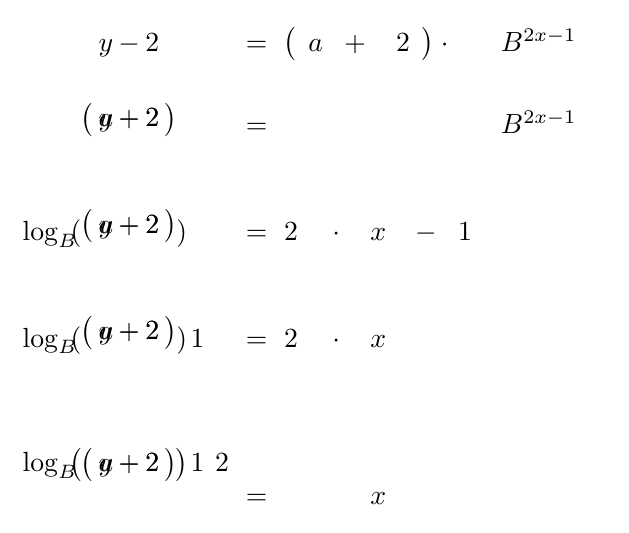
\begin{tikzpicture}[x=1em,y=-1em]
\node[anchor=base, inner sep=0pt] at (18.47,2.72) {$\pFourCell{4.46}{B^{{\scriptstyle 2x-1}}}$};
\node[anchor=base, inner sep=0pt] at (2.83,2.72) {$\pFourCell{0.9}{y}$};
\node[anchor=base, inner sep=0pt] at (3.67,2.72) {$\pFourCell{0.78}{-}$};
\node[anchor=base, inner sep=0pt] at (4.5,2.72) {$\pFourCell{0.88}{2}$};
\node[anchor=base, inner sep=0pt] at (8.27,2.72) {$\pFourCell{1.62}{=}$};
\node[anchor=base, inner sep=0pt] at (9.52,2.72) {$\pFourCell{0.88}{\left(\rule[-0.32em]{0pt}{0.84em}\right.}$};
\node[anchor=base, inner sep=0pt] at (10.41,2.72) {$\pFourCell{0.9}{a}$};
\node[anchor=base, inner sep=0pt] at (11.83,2.72) {$\pFourCell{0.78}{+}$};
\node[anchor=base, inner sep=0pt] at (13.56,2.72) {$\pFourCell{0.88}{2}$};
\node[anchor=base, inner sep=0pt] at (14.39,2.72) {$\pFourCell{0.78}{\left.\rule[-0.32em]{0pt}{0.84em}\right)}$};
\node[anchor=base, inner sep=0pt] at (15.07,2.72) {$\pFourCell{0.58}{\cdot{}}$};
\node[anchor=base, inner sep=0pt] at (18.47,5.71) {$\pFourCell{4.46}{B^{{\scriptstyle 2x-1}}}$};
\node[anchor=base, inner sep=0pt] at (2.83,5.44) {$\pFourCell{0.9}{y}$};
\node[anchor=base, inner sep=0pt] at (3.67,5.44) {$\pFourCell{0.78}{-}$};
\node[anchor=base, inner sep=0pt] at (4.5,5.44) {$\pFourCell{0.88}{2}$};
\node[anchor=base, inner sep=0pt] at (8.27,5.71) {$\pFourCell{1.62}{=}$};
\node[anchor=base, inner sep=0pt] at (2.19,5.44) {$\pFourCell{0.38}{\left(\rule[-0.32em]{0pt}{0.84em}\right.}$};
\node[anchor=base, inner sep=0pt] at (2.83,5.44) {$\pFourCell{0.9}{a}$};
\node[anchor=base, inner sep=0pt] at (3.67,5.44) {$\pFourCell{0.78}{+}$};
\node[anchor=base, inner sep=0pt] at (4.5,5.44) {$\pFourCell{0.88}{2}$};
\node[anchor=base, inner sep=0pt] at (5.13,5.44) {$\pFourCell{0.38}{\left.\rule[-0.32em]{0pt}{0.84em}\right)}$};
\node[anchor=base, inner sep=0pt] at (2.83,9.29) {$\pFourCell{0.9}{y}$};
\node[anchor=base, inner sep=0pt] at (3.67,9.29) {$\pFourCell{0.78}{-}$};
\node[anchor=base, inner sep=0pt] at (4.5,9.29) {$\pFourCell{0.88}{2}$};
\node[anchor=base, inner sep=0pt] at (0.81,9.56) {$\pFourCell{1.62}{\log_{B}}$};
\node[anchor=base, inner sep=0pt] at (1.81,9.56) {$\pFourCell{0.38}{\left(\rule[-0.28em]{0pt}{1.07em}\right.}$};
\node[anchor=base, inner sep=0pt] at (5.51,9.56) {$\pFourCell{0.38}{\left.\rule[-0.28em]{0pt}{1.07em}\right)}$};
\node[anchor=base, inner sep=0pt] at (8.27,9.56) {$\pFourCell{1.62}{=}$};
\node[anchor=base, inner sep=0pt] at (9.52,9.56) {$\pFourCell{0.88}{2}$};
\node[anchor=base, inner sep=0pt] at (11.15,9.56) {$\pFourCell{0.58}{\cdot{}}$};
\node[anchor=base, inner sep=0pt] at (12.67,9.56) {$\pFourCell{0.9}{x}$};
\node[anchor=base, inner sep=0pt] at (14.39,9.56) {$\pFourCell{0.78}{-}$};
\node[anchor=base, inner sep=0pt] at (15.8,9.56) {$\pFourCell{0.88}{1}$};
\node[anchor=base, inner sep=0pt] at (2.19,9.29) {$\pFourCell{0.38}{\left(\rule[-0.32em]{0pt}{0.84em}\right.}$};
\node[anchor=base, inner sep=0pt] at (2.83,9.29) {$\pFourCell{0.9}{a}$};
\node[anchor=base, inner sep=0pt] at (3.67,9.29) {$\pFourCell{0.78}{+}$};
\node[anchor=base, inner sep=0pt] at (4.5,9.29) {$\pFourCell{0.88}{2}$};
\node[anchor=base, inner sep=0pt] at (5.13,9.29) {$\pFourCell{0.38}{\left.\rule[-0.32em]{0pt}{0.84em}\right)}$};
\node[anchor=base, inner sep=0pt] at (2.83,13.14) {$\pFourCell{0.9}{y}$};
\node[anchor=base, inner sep=0pt] at (3.67,13.14) {$\pFourCell{0.78}{-}$};
\node[anchor=base, inner sep=0pt] at (4.5,13.14) {$\pFourCell{0.88}{2}$};
\node[anchor=base, inner sep=0pt] at (0.81,13.41) {$\pFourCell{1.62}{\log_{B}}$};
\node[anchor=base, inner sep=0pt] at (1.81,13.41) {$\pFourCell{0.38}{\left(\rule[-0.28em]{0pt}{1.07em}\right.}$};
\node[anchor=base, inner sep=0pt] at (5.51,13.41) {$\pFourCell{0.38}{\left.\rule[-0.28em]{0pt}{1.07em}\right)}$};
\node[anchor=base, inner sep=0pt] at (6.14,13.41) {$\pFourCell{0.88}{1}$};
\node[anchor=base, inner sep=0pt] at (8.27,13.41) {$\pFourCell{1.62}{=}$};
\node[anchor=base, inner sep=0pt] at (9.52,13.41) {$\pFourCell{0.88}{2}$};
\node[anchor=base, inner sep=0pt] at (11.15,13.41) {$\pFourCell{0.58}{\cdot{}}$};
\node[anchor=base, inner sep=0pt] at (12.67,13.41) {$\pFourCell{0.9}{x}$};
\node[anchor=base, inner sep=0pt] at (2.19,13.14) {$\pFourCell{0.38}{\left(\rule[-0.32em]{0pt}{0.84em}\right.}$};
\node[anchor=base, inner sep=0pt] at (2.83,13.14) {$\pFourCell{0.9}{a}$};
\node[anchor=base, inner sep=0pt] at (3.67,13.14) {$\pFourCell{0.78}{+}$};
\node[anchor=base, inner sep=0pt] at (4.5,13.14) {$\pFourCell{0.88}{2}$};
\node[anchor=base, inner sep=0pt] at (5.13,13.14) {$\pFourCell{0.38}{\left.\rule[-0.32em]{0pt}{0.84em}\right)}$};
\node[anchor=base, inner sep=0pt] at (2.83,17.91) {$\pFourCell{0.9}{y}$};
\node[anchor=base, inner sep=0pt] at (3.67,17.91) {$\pFourCell{0.78}{-}$};
\node[anchor=base, inner sep=0pt] at (4.5,17.91) {$\pFourCell{0.88}{2}$};
\node[anchor=base, inner sep=0pt] at (0.81,17.91) {$\pFourCell{1.62}{\log_{B}}$};
\node[anchor=base, inner sep=0pt] at (1.81,17.91) {$\pFourCell{0.38}{\left(\rule[-0.32em]{0pt}{0.84em}\right.}$};
\node[anchor=base, inner sep=0pt] at (2.19,17.91) {$\pFourCell{0.38}{\left(\rule[-0.32em]{0pt}{0.84em}\right.}$};
\node[anchor=base, inner sep=0pt] at (2.83,17.91) {$\pFourCell{0.9}{a}$};
\node[anchor=base, inner sep=0pt] at (3.67,17.91) {$\pFourCell{0.78}{+}$};
\node[anchor=base, inner sep=0pt] at (4.5,17.91) {$\pFourCell{0.88}{2}$};
\node[anchor=base, inner sep=0pt] at (5.13,17.91) {$\pFourCell{0.38}{\left.\rule[-0.32em]{0pt}{0.84em}\right)}$};
\node[anchor=base, inner sep=0pt] at (5.51,17.91) {$\pFourCell{0.38}{\left.\rule[-0.32em]{0pt}{0.84em}\right)}$};
\node[anchor=base, inner sep=0pt] at (6.14,17.91) {$\pFourCell{0.88}{1}$};
\node[anchor=base, inner sep=0pt] at (8.27,19.1) {$\pFourCell{1.62}{=}$};
\node[anchor=base, inner sep=0pt] at (12.67,19.1) {$\pFourCell{0.9}{x}$};
\node[anchor=base, inner sep=0pt] at (7.02,17.91) {$\pFourCell{0.88}{2}$};
\end{tikzpicture}
\end{center}


\newpage
\section*{Spaltentreue LaTeX-Ausgabe mit Spaltengrenzen}
\vspace{6mm}
\begin{center}
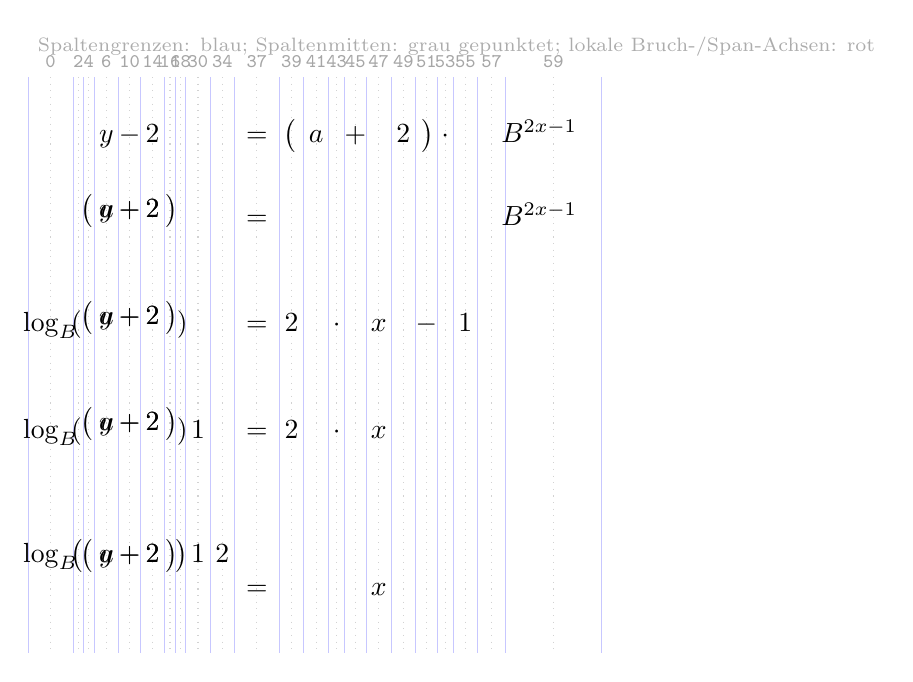
\begin{tikzpicture}[x=1em,y=-1em]
\node[font={\scriptsize}, text=gray!65, anchor=west] at (0,-0.75) {Spaltengrenzen: blau; Spaltenmitten: grau gepunktet; lokale Bruch-/Span-Achsen: rot};
\draw[blue!22, line width=0.28pt] (0,0.35) -- (0,21.18);
\draw[blue!22, line width=0.28pt] (1.62,0.35) -- (1.62,21.18);
\draw[blue!22, line width=0.28pt] (2,0.35) -- (2,21.18);
\draw[blue!22, line width=0.28pt] (2.38,0.35) -- (2.38,21.18);
\draw[blue!22, line width=0.28pt] (3.28,0.35) -- (3.28,21.18);
\draw[blue!22, line width=0.28pt] (4.06,0.35) -- (4.06,21.18);
\draw[blue!22, line width=0.28pt] (4.94,0.35) -- (4.94,21.18);
\draw[blue!22, line width=0.28pt] (5.32,0.35) -- (5.32,21.18);
\draw[blue!22, line width=0.28pt] (5.7,0.35) -- (5.7,21.18);
\draw[blue!22, line width=0.28pt] (6.58,0.35) -- (6.58,21.18);
\draw[blue!22, line width=0.28pt] (7.46,0.35) -- (7.46,21.18);
\draw[blue!22, line width=0.28pt] (9.08,0.35) -- (9.08,21.18);
\draw[blue!22, line width=0.28pt] (9.96,0.35) -- (9.96,21.18);
\draw[blue!22, line width=0.28pt] (10.86,0.35) -- (10.86,21.18);
\draw[blue!22, line width=0.28pt] (11.44,0.35) -- (11.44,21.18);
\draw[blue!22, line width=0.28pt] (12.22,0.35) -- (12.22,21.18);
\draw[blue!22, line width=0.28pt] (13.12,0.35) -- (13.12,21.18);
\draw[blue!22, line width=0.28pt] (14,0.35) -- (14,21.18);
\draw[blue!22, line width=0.28pt] (14.78,0.35) -- (14.78,21.18);
\draw[blue!22, line width=0.28pt] (15.36,0.35) -- (15.36,21.18);
\draw[blue!22, line width=0.28pt] (16.24,0.35) -- (16.24,21.18);
\draw[blue!22, line width=0.28pt] (17.26,0.35) -- (17.26,21.18);
\draw[blue!22, line width=0.28pt] (20.7,0.35) -- (20.7,21.18);
\draw[gray!35, dotted] (0.81,0.35) -- (0.81,21.18);
\node[font={\ttfamily\scriptsize}, text=gray!70, anchor=base] at (0.81,0) {0};
\draw[gray!35, dotted] (1.81,0.35) -- (1.81,21.18);
\node[font={\ttfamily\scriptsize}, text=gray!70, anchor=base] at (1.81,0) {2};
\draw[gray!35, dotted] (2.19,0.35) -- (2.19,21.18);
\node[font={\ttfamily\scriptsize}, text=gray!70, anchor=base] at (2.19,0) {4};
\draw[gray!35, dotted] (2.83,0.35) -- (2.83,21.18);
\node[font={\ttfamily\scriptsize}, text=gray!70, anchor=base] at (2.83,0) {6};
\draw[gray!35, dotted] (3.67,0.35) -- (3.67,21.18);
\node[font={\ttfamily\scriptsize}, text=gray!70, anchor=base] at (3.67,0) {10};
\draw[gray!35, dotted] (4.5,0.35) -- (4.5,21.18);
\node[font={\ttfamily\scriptsize}, text=gray!70, anchor=base] at (4.5,0) {14};
\draw[gray!35, dotted] (5.13,0.35) -- (5.13,21.18);
\node[font={\ttfamily\scriptsize}, text=gray!70, anchor=base] at (5.13,0) {16};
\draw[gray!35, dotted] (5.51,0.35) -- (5.51,21.18);
\node[font={\ttfamily\scriptsize}, text=gray!70, anchor=base] at (5.51,0) {18};
\draw[gray!35, dotted] (6.14,0.35) -- (6.14,21.18);
\node[font={\ttfamily\scriptsize}, text=gray!70, anchor=base] at (6.14,0) {30};
\draw[gray!35, dotted] (7.02,0.35) -- (7.02,21.18);
\node[font={\ttfamily\scriptsize}, text=gray!70, anchor=base] at (7.02,0) {34};
\draw[gray!35, dotted] (8.27,0.35) -- (8.27,21.18);
\node[font={\ttfamily\scriptsize}, text=gray!70, anchor=base] at (8.27,0) {37};
\draw[gray!35, dotted] (9.52,0.35) -- (9.52,21.18);
\node[font={\ttfamily\scriptsize}, text=gray!70, anchor=base] at (9.52,0) {39};
\draw[gray!35, dotted] (10.41,0.35) -- (10.41,21.18);
\node[font={\ttfamily\scriptsize}, text=gray!70, anchor=base] at (10.41,0) {41};
\draw[gray!35, dotted] (11.15,0.35) -- (11.15,21.18);
\node[font={\ttfamily\scriptsize}, text=gray!70, anchor=base] at (11.15,0) {43};
\draw[gray!35, dotted] (11.83,0.35) -- (11.83,21.18);
\node[font={\ttfamily\scriptsize}, text=gray!70, anchor=base] at (11.83,0) {45};
\draw[gray!35, dotted] (12.67,0.35) -- (12.67,21.18);
\node[font={\ttfamily\scriptsize}, text=gray!70, anchor=base] at (12.67,0) {47};
\draw[gray!35, dotted] (13.56,0.35) -- (13.56,21.18);
\node[font={\ttfamily\scriptsize}, text=gray!70, anchor=base] at (13.56,0) {49};
\draw[gray!35, dotted] (14.39,0.35) -- (14.39,21.18);
\node[font={\ttfamily\scriptsize}, text=gray!70, anchor=base] at (14.39,0) {51};
\draw[gray!35, dotted] (15.07,0.35) -- (15.07,21.18);
\node[font={\ttfamily\scriptsize}, text=gray!70, anchor=base] at (15.07,0) {53};
\draw[gray!35, dotted] (15.8,0.35) -- (15.8,21.18);
\node[font={\ttfamily\scriptsize}, text=gray!70, anchor=base] at (15.8,0) {55};
\draw[gray!35, dotted] (16.75,0.35) -- (16.75,21.18);
\node[font={\ttfamily\scriptsize}, text=gray!70, anchor=base] at (16.75,0) {57};
\draw[gray!35, dotted] (18.98,0.35) -- (18.98,21.18);
\node[font={\ttfamily\scriptsize}, text=gray!70, anchor=base] at (18.98,0) {59};
\node[anchor=base, inner sep=0pt] at (18.47,2.72) {$\pFourCell{4.46}{B^{{\scriptstyle 2x-1}}}$};
\node[anchor=base, inner sep=0pt] at (2.83,2.72) {$\pFourCell{0.9}{y}$};
\node[anchor=base, inner sep=0pt] at (3.67,2.72) {$\pFourCell{0.78}{-}$};
\node[anchor=base, inner sep=0pt] at (4.5,2.72) {$\pFourCell{0.88}{2}$};
\node[anchor=base, inner sep=0pt] at (8.27,2.72) {$\pFourCell{1.62}{=}$};
\node[anchor=base, inner sep=0pt] at (9.52,2.72) {$\pFourCell{0.88}{\left(\rule[-0.32em]{0pt}{0.84em}\right.}$};
\node[anchor=base, inner sep=0pt] at (10.41,2.72) {$\pFourCell{0.9}{a}$};
\node[anchor=base, inner sep=0pt] at (11.83,2.72) {$\pFourCell{0.78}{+}$};
\node[anchor=base, inner sep=0pt] at (13.56,2.72) {$\pFourCell{0.88}{2}$};
\node[anchor=base, inner sep=0pt] at (14.39,2.72) {$\pFourCell{0.78}{\left.\rule[-0.32em]{0pt}{0.84em}\right)}$};
\node[anchor=base, inner sep=0pt] at (15.07,2.72) {$\pFourCell{0.58}{\cdot{}}$};
\node[anchor=base, inner sep=0pt] at (18.47,5.71) {$\pFourCell{4.46}{B^{{\scriptstyle 2x-1}}}$};
\node[anchor=base, inner sep=0pt] at (2.83,5.44) {$\pFourCell{0.9}{y}$};
\node[anchor=base, inner sep=0pt] at (3.67,5.44) {$\pFourCell{0.78}{-}$};
\node[anchor=base, inner sep=0pt] at (4.5,5.44) {$\pFourCell{0.88}{2}$};
\node[anchor=base, inner sep=0pt] at (8.27,5.71) {$\pFourCell{1.62}{=}$};
\node[anchor=base, inner sep=0pt] at (2.19,5.44) {$\pFourCell{0.38}{\left(\rule[-0.32em]{0pt}{0.84em}\right.}$};
\node[anchor=base, inner sep=0pt] at (2.83,5.44) {$\pFourCell{0.9}{a}$};
\node[anchor=base, inner sep=0pt] at (3.67,5.44) {$\pFourCell{0.78}{+}$};
\node[anchor=base, inner sep=0pt] at (4.5,5.44) {$\pFourCell{0.88}{2}$};
\node[anchor=base, inner sep=0pt] at (5.13,5.44) {$\pFourCell{0.38}{\left.\rule[-0.32em]{0pt}{0.84em}\right)}$};
\node[anchor=base, inner sep=0pt] at (2.83,9.29) {$\pFourCell{0.9}{y}$};
\node[anchor=base, inner sep=0pt] at (3.67,9.29) {$\pFourCell{0.78}{-}$};
\node[anchor=base, inner sep=0pt] at (4.5,9.29) {$\pFourCell{0.88}{2}$};
\node[anchor=base, inner sep=0pt] at (0.81,9.56) {$\pFourCell{1.62}{\log_{B}}$};
\node[anchor=base, inner sep=0pt] at (1.81,9.56) {$\pFourCell{0.38}{\left(\rule[-0.28em]{0pt}{1.07em}\right.}$};
\node[anchor=base, inner sep=0pt] at (5.51,9.56) {$\pFourCell{0.38}{\left.\rule[-0.28em]{0pt}{1.07em}\right)}$};
\node[anchor=base, inner sep=0pt] at (8.27,9.56) {$\pFourCell{1.62}{=}$};
\node[anchor=base, inner sep=0pt] at (9.52,9.56) {$\pFourCell{0.88}{2}$};
\node[anchor=base, inner sep=0pt] at (11.15,9.56) {$\pFourCell{0.58}{\cdot{}}$};
\node[anchor=base, inner sep=0pt] at (12.67,9.56) {$\pFourCell{0.9}{x}$};
\node[anchor=base, inner sep=0pt] at (14.39,9.56) {$\pFourCell{0.78}{-}$};
\node[anchor=base, inner sep=0pt] at (15.8,9.56) {$\pFourCell{0.88}{1}$};
\node[anchor=base, inner sep=0pt] at (2.19,9.29) {$\pFourCell{0.38}{\left(\rule[-0.32em]{0pt}{0.84em}\right.}$};
\node[anchor=base, inner sep=0pt] at (2.83,9.29) {$\pFourCell{0.9}{a}$};
\node[anchor=base, inner sep=0pt] at (3.67,9.29) {$\pFourCell{0.78}{+}$};
\node[anchor=base, inner sep=0pt] at (4.5,9.29) {$\pFourCell{0.88}{2}$};
\node[anchor=base, inner sep=0pt] at (5.13,9.29) {$\pFourCell{0.38}{\left.\rule[-0.32em]{0pt}{0.84em}\right)}$};
\node[anchor=base, inner sep=0pt] at (2.83,13.14) {$\pFourCell{0.9}{y}$};
\node[anchor=base, inner sep=0pt] at (3.67,13.14) {$\pFourCell{0.78}{-}$};
\node[anchor=base, inner sep=0pt] at (4.5,13.14) {$\pFourCell{0.88}{2}$};
\node[anchor=base, inner sep=0pt] at (0.81,13.41) {$\pFourCell{1.62}{\log_{B}}$};
\node[anchor=base, inner sep=0pt] at (1.81,13.41) {$\pFourCell{0.38}{\left(\rule[-0.28em]{0pt}{1.07em}\right.}$};
\node[anchor=base, inner sep=0pt] at (5.51,13.41) {$\pFourCell{0.38}{\left.\rule[-0.28em]{0pt}{1.07em}\right)}$};
\node[anchor=base, inner sep=0pt] at (6.14,13.41) {$\pFourCell{0.88}{1}$};
\node[anchor=base, inner sep=0pt] at (8.27,13.41) {$\pFourCell{1.62}{=}$};
\node[anchor=base, inner sep=0pt] at (9.52,13.41) {$\pFourCell{0.88}{2}$};
\node[anchor=base, inner sep=0pt] at (11.15,13.41) {$\pFourCell{0.58}{\cdot{}}$};
\node[anchor=base, inner sep=0pt] at (12.67,13.41) {$\pFourCell{0.9}{x}$};
\node[anchor=base, inner sep=0pt] at (2.19,13.14) {$\pFourCell{0.38}{\left(\rule[-0.32em]{0pt}{0.84em}\right.}$};
\node[anchor=base, inner sep=0pt] at (2.83,13.14) {$\pFourCell{0.9}{a}$};
\node[anchor=base, inner sep=0pt] at (3.67,13.14) {$\pFourCell{0.78}{+}$};
\node[anchor=base, inner sep=0pt] at (4.5,13.14) {$\pFourCell{0.88}{2}$};
\node[anchor=base, inner sep=0pt] at (5.13,13.14) {$\pFourCell{0.38}{\left.\rule[-0.32em]{0pt}{0.84em}\right)}$};
\node[anchor=base, inner sep=0pt] at (2.83,17.91) {$\pFourCell{0.9}{y}$};
\node[anchor=base, inner sep=0pt] at (3.67,17.91) {$\pFourCell{0.78}{-}$};
\node[anchor=base, inner sep=0pt] at (4.5,17.91) {$\pFourCell{0.88}{2}$};
\node[anchor=base, inner sep=0pt] at (0.81,17.91) {$\pFourCell{1.62}{\log_{B}}$};
\node[anchor=base, inner sep=0pt] at (1.81,17.91) {$\pFourCell{0.38}{\left(\rule[-0.32em]{0pt}{0.84em}\right.}$};
\node[anchor=base, inner sep=0pt] at (2.19,17.91) {$\pFourCell{0.38}{\left(\rule[-0.32em]{0pt}{0.84em}\right.}$};
\node[anchor=base, inner sep=0pt] at (2.83,17.91) {$\pFourCell{0.9}{a}$};
\node[anchor=base, inner sep=0pt] at (3.67,17.91) {$\pFourCell{0.78}{+}$};
\node[anchor=base, inner sep=0pt] at (4.5,17.91) {$\pFourCell{0.88}{2}$};
\node[anchor=base, inner sep=0pt] at (5.13,17.91) {$\pFourCell{0.38}{\left.\rule[-0.32em]{0pt}{0.84em}\right)}$};
\node[anchor=base, inner sep=0pt] at (5.51,17.91) {$\pFourCell{0.38}{\left.\rule[-0.32em]{0pt}{0.84em}\right)}$};
\node[anchor=base, inner sep=0pt] at (6.14,17.91) {$\pFourCell{0.88}{1}$};
\node[anchor=base, inner sep=0pt] at (8.27,19.1) {$\pFourCell{1.62}{=}$};
\node[anchor=base, inner sep=0pt] at (12.67,19.1) {$\pFourCell{0.9}{x}$};
\node[anchor=base, inner sep=0pt] at (7.02,17.91) {$\pFourCell{0.88}{2}$};
\end{tikzpicture}
\end{center}
\end{document}
